\section{Simbol Flowchart Standar}

Berdasarkan standar ANSI dan referensi dari Lucidchart, simbol flowchart standar meliputi beberapa jenis dengan fungsi spesifik \cite{flowchart_lucidchart}. Setiap simbol dirancang untuk merepresentasikan jenis operasi tertentu dalam algoritma.

\subsection{Simbol-Simbol Dasar}

\begin{table}[htbp]
\centering
\small
\begin{tabular}{|>{\raggedright\arraybackslash}p{2.5cm}|>{\raggedright\arraybackslash}p{2.5cm}|>{\raggedright\arraybackslash}p{6cm}|}
\hline
\textbf{Simbol} & \textbf{Nama} & \textbf{Fungsi dan Contoh} \\
\hline
Oval & Terminator & Mulai/Akhir program. Contoh: "Start", "End" \\
\hline
Persegi Panjang & Proses & Operasi, perhitungan, penugasan. Contoh: "x = x + 1" \\
\hline
Belah Ketupat & Keputusan & Percabangan (Ya/Tidak). Contoh: "x > 0?" \\
\hline
Jajar Genjang & Input/Output & Membaca input atau menampilkan output. Contoh: "Input nilai", "Print hasil" \\
\hline
Panah & Garis Alur & Menunjukkan urutan eksekusi program \\
\hline
\end{tabular}
\caption{Simbol Flowchart Dasar}
\end{table}

\subsection{Simbol Tambahan}

\begin{table}[htbp]
\centering
\small
\begin{tabular}{|>{\raggedright\arraybackslash}p{2.5cm}|>{\raggedright\arraybackslash}p{2.5cm}|>{\raggedright\arraybackslash}p{6cm}|}
\hline
\textbf{Simbol} & \textbf{Nama} & \textbf{Fungsi dan Contoh} \\
\hline
Persegi Panjang Ganda & Preparasi & Persiapan atau inisialisasi. Contoh: "Inisialisasi variabel" \\
\hline
Hexagon & Loop & Awal dan akhir loop. Contoh: "For i = 1 to 10" \\
\hline
Lingkaran & Connector & Menghubungkan bagian flowchart yang sama halaman \\
\hline
Persegi Rumah & Off-page & Menghubungkan flowchart antar halaman \\
\hline
Garis Putus-putus & Comment & Komentar atau penjelasan tambahan \\
\hline
Dokumen & Data & Input/output dokumen. Contoh: "Baca file data.txt" \\
\hline
\end{tabular}
\caption{Simbol Flowchart Tambahan}
\end{table}

\subsection{Contoh Visual Simbol Flowchart}

Berikut adalah representasi visual dari simbol-simbol flowchart utama:

\begin{center}
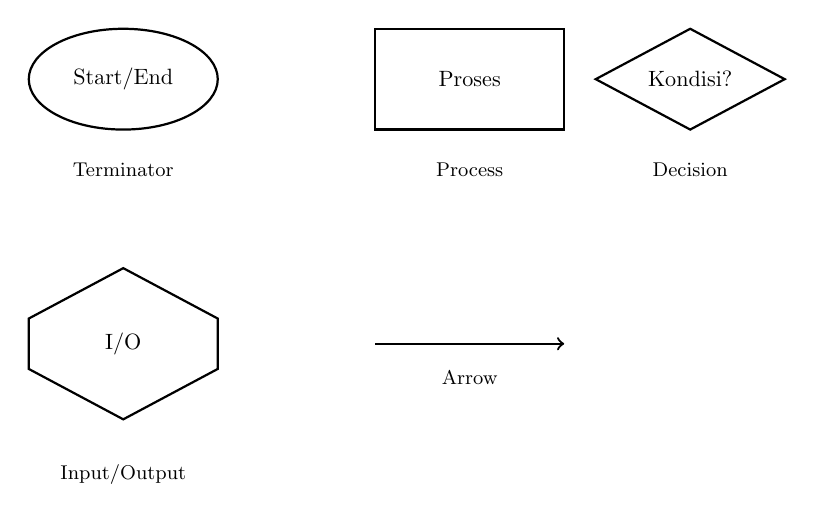
\begin{tikzpicture}[scale=0.8, transform shape]
  % Terminator
  \draw[thick] (0,0) ellipse (1.5cm and 0.8cm);
  \node at (0,0) {Start/End};
  \node[below] at (0,-1.2) {\small Terminator};
  
  % Process
  \draw[thick] (4,0.8) rectangle (7,-0.8);
  \node at (5.5,0) {Proses};
  \node[below] at (5.5,-1.2) {\small Process};
  
  % Decision
  \draw[thick] (9,0.8) -- (10.5,0) -- (9,-0.8) -- (7.5,0) -- cycle;
  \node at (9,0) {Kondisi?};
  \node[below] at (9,-1.2) {\small Decision};
  
  % Input/Output
  \draw[thick] (0,-3) -- (1.5,-3.8) -- (1.5,-4.6) -- (0,-5.4) -- (-1.5,-4.6) -- (-1.5,-3.8) -- cycle;
  \node at (0,-4.2) {I/O};
  \node[below] at (0,-6) {\small Input/Output};
  
  % Arrow
  \draw[thick, ->] (4,-4.2) -- (7,-4.2);
  \node[below] at (5.5,-4.5) {\small Arrow};
\end{tikzpicture}
\end{center}

\subsection{Aturan Penggunaan Simbol}

\begin{itemize}
  \item \textbf{Konsistensi:} Gunakan simbol yang sama untuk operasi yang sama di seluruh flowchart
  \item \textbf{Keterbacaan:} Pastikan teks di dalam simbol mudah dibaca dan singkat
  \item \textbf{Arah Alur:} Gunakan panah untuk menunjukkan arah alur yang jelas
  \item \textbf{Hierarki:} Simbol utama (terminator) selalu di bagian atas atau bawah
  \item \textbf{Koneksi:} Gunakan connector untuk flowchart yang kompleks
\end{itemize}

Pemahaman yang baik tentang simbol-simbol ini menjadi fondasi untuk membuat flowchart yang efektif dan sesuai standar industri.
